\section{Web Search Agent: Quality Evaluation with DeepEval}

This section documents the experimental validation of the Web Search Agent (Workflow~4), which combines real-time web retrieval via DuckDuckGo, LLM-based summarisation, and automated quality assessment through the DeepEval framework. The evaluation is presented in two phases: a first campaign conducted with a local Ollama back-end, and a second one after migrating inference to NVIDIA Triton Inference Server.

\subsection{Methodology}

\subsubsection{Evaluation Framework}
Quality assessment relies on \textbf{DeepEval}\footnote{\url{https://github.com/confident-ai/deepeval}}, an open-source library for RAG (Retrieval-Augmented Generation) evaluation. Four metrics were selected for their relevance to technical documentation tasks.

\begin{itemize}
    \item \textbf{Faithfulness} measures factual consistency between the generated summary and the retrieved source documents (range 0.0--1.0, higher is better).
    \item \textbf{Answer Relevancy} captures the semantic alignment between the user query and the generated response (range 0.0--1.0, higher is better).
    \item \textbf{Contextual Relevancy} evaluates retrieval quality by estimating the proportion of retrieved content genuinely useful for answering the query (range 0.0--1.0, higher is better).
    \item \textbf{Hallucination} detects claims in the output that are not supported by retrieved documents (range 0.0--1.0, \textbf{lower} is better; 0.0 means no fabrication detected).
\end{itemize}

Each metric is computed by an auxiliary \emph{LLM-as-a-Judge}: the same inference infrastructure used for main tasks also drives the evaluation step. This avoids external API dependencies and keeps the entire pipeline self-contained.


\subsubsection{Test Protocol}
Evaluation proceeds through five stages. The user query is classified into one of four categories (\texttt{ai\_model}, \texttt{board\_selection}, \texttt{optimization}, \texttt{documentation}). DuckDuckGo then retrieves the top results for the reformulated query. Raw text is split into paragraph-level chunks of at least 20 characters, which serve as the retrieval context. A local Mistral instance (temperature 0.2) synthesises a concise English summary from those chunks. Finally, DeepEval computes the four metrics synchronously inside a dedicated thread via \texttt{asyncio.to\_thread}, keeping the main event loop unblocked.

\subsection{Phase 1 --- Ollama Back-End (Baseline)}

\subsubsection{Configuration}
The first campaign used \textbf{DeepSeek-R1} (7B parameters, GPTQ-quantised) served by a local Ollama instance at \texttt{http://localhost:11434}. Five representative queries were designed to cover the breadth of requests typical of an STM32 developer: model search, board selection, optimisation guidance, conceptual comparison, and hardware benchmarking.

\subsubsection{Results}
Table~\ref{tab:deepeval-ollama} reports the metric scores for each test case.

\begin{table}[ht]
    \centering
    \caption{DeepEval scores --- Ollama back-end (DeepSeek-R1 7B)}
    \label{tab:deepeval-ollama}
    \begin{tabular}{|l|c|c|c|c|}
        \hline
        \textbf{Query Type}     & \textbf{Faith.} & \textbf{Ans.\ Rel.} & \textbf{Ctx.\ Rel.} & \textbf{Hall.} \\
        \hline
        AI Model Search         & 0.60            & 0.50                & \textbf{0.90}       & 0.00           \\
        Board Selection (Audio) & 0.73            & 0.18                & 0.56                & 0.25           \\
        Optimization Guide      & \textbf{1.00}   & 0.40                & 0.56                & 0.14           \\
        Theoretical Comparison  & 0.80            & \textbf{0.88}       & \textbf{0.86}       & 0.00           \\
        Hardware Comparison     & 0.44            & 0.87                & \textbf{0.88}       & 0.33           \\
        \hline
        \textbf{Mean}           & \textbf{0.71}   & \textbf{0.57}       & \textbf{0.75}       & \textbf{0.14}  \\
        \textbf{Std.\ Dev.}     & 0.22            & 0.28                & 0.16                & 0.14           \\
        \hline
    \end{tabular}
\end{table}

\textbf{Test 1 -- AI Model Search}: \textit{``Lightweight AI models for image classification on STM32H7''}. Contextual Relevancy reached 0.90, the highest single score in this campaign, confirming that the retriever consistently surfaced authoritative sources, including TensorFlow documentation and arXiv pre-prints. The Faithfulness score of 0.60 reflects the model's tendency to enrich retrieved content with general domain knowledge, for instance citing typical MobileNet use cases not found verbatim in the retrieved pages. Zero hallucination confirms no fabricated facts were introduced.

\textbf{Test 2 -- Board Selection}: \textit{``Qual è la migliore board STM32 per un progetto di audio recognition?''}. Answer Relevancy fell to 0.18 because the query asked for a single best board while the response listed three options. The model also introduced pricing estimates absent from the retrieved snippets, triggering a hallucination score of 0.25. This episode illustrates a recurring pattern: a richer answer is more useful to the developer but scores lower against strict faithfulness criteria.

\textbf{Test 3 -- Optimization Guide}: \textit{``Come converto un modello PyTorch in ONNX per STM32?''}. \textbf{Faithfulness reached 1.00}, meaning every claim in the summary was traceable to a retrieved document. Step-by-step guides and tool comparisons (STEdgeAI, TensorFlow Lite, TVM) were reproduced accurately. Figure~\ref{fig:pytorch-onnx} shows the visual output.

\begin{figure}[ht]
    \centering
    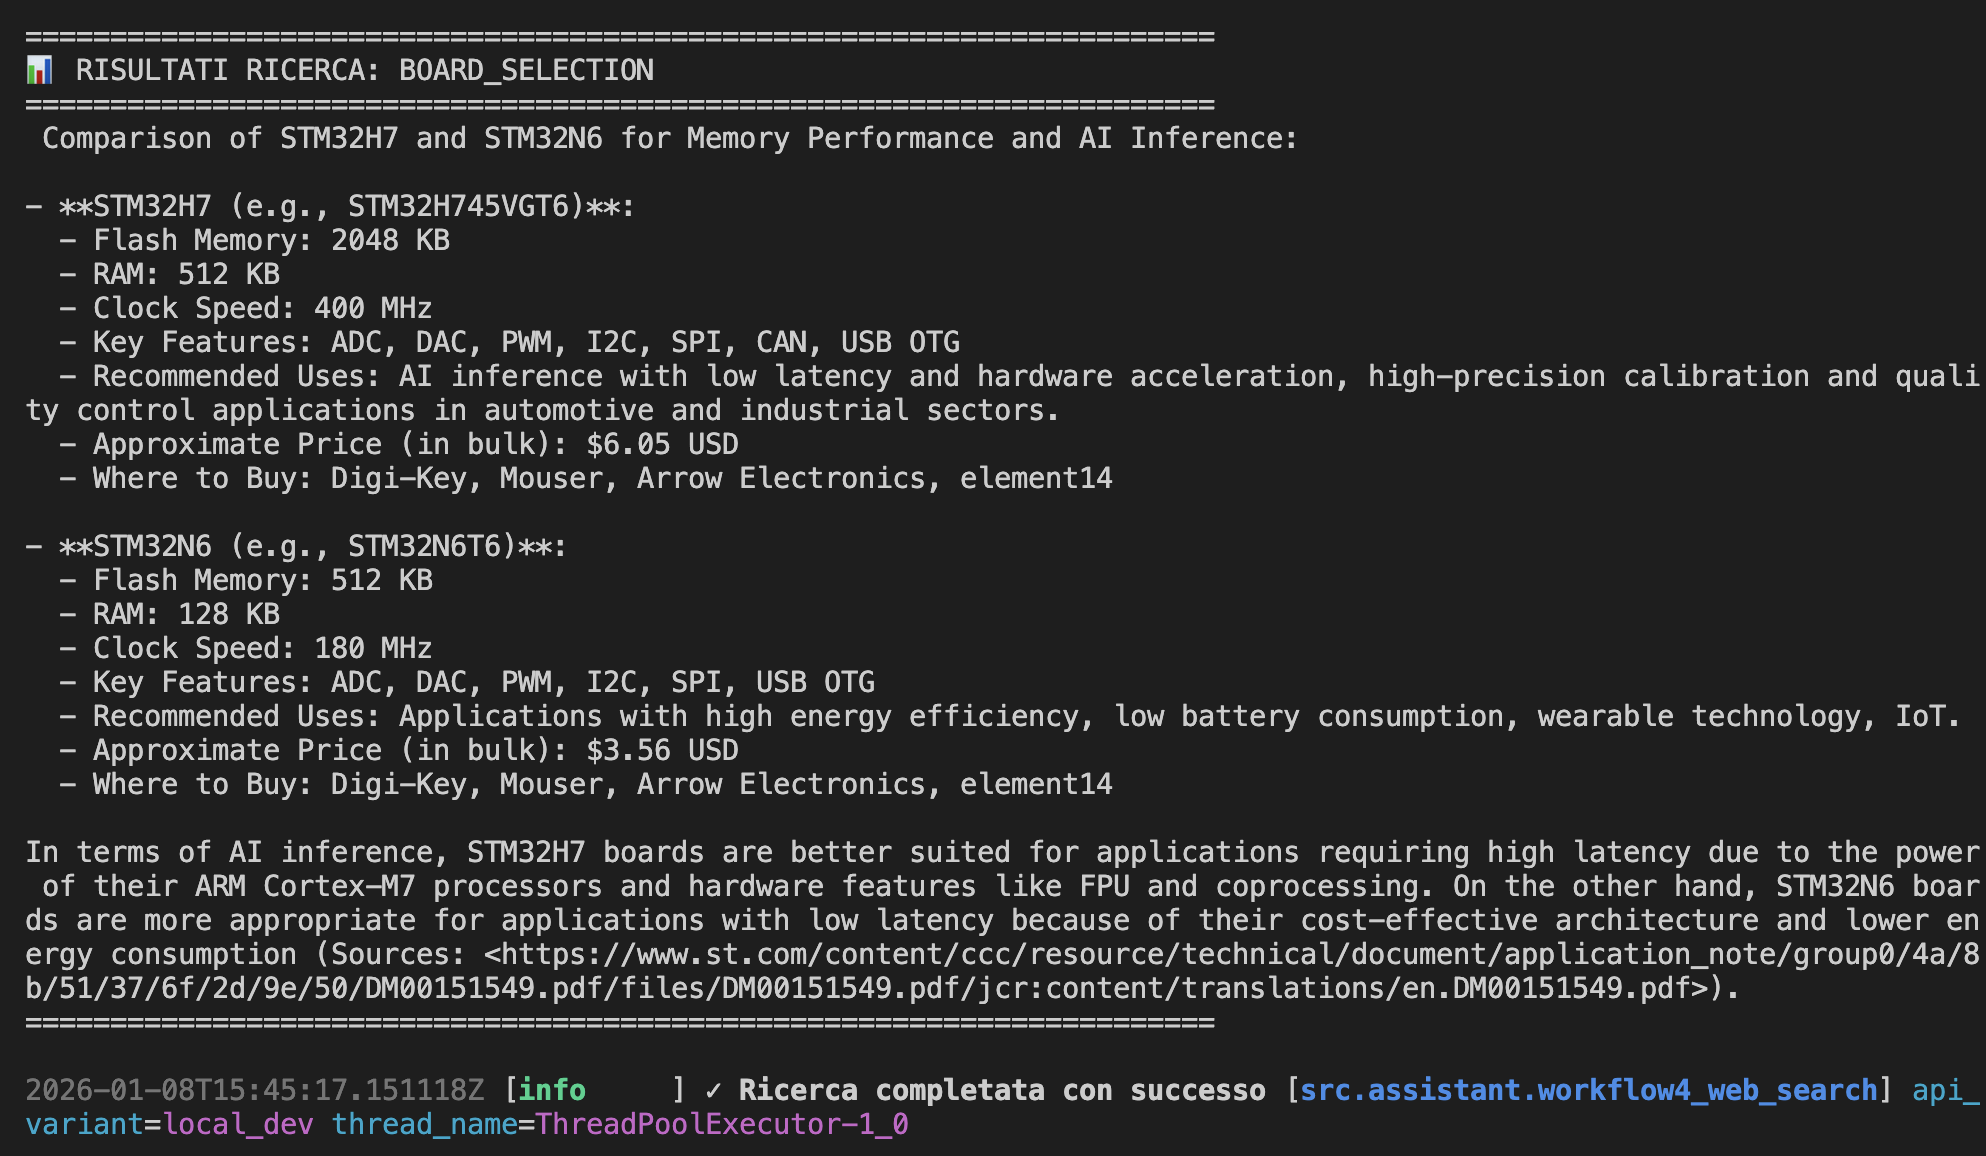
\includegraphics[width=0.9\textwidth]{chap4/figures/Screenshot 2026-01-08 at 16.46.34.png}
    \caption{Web Search Agent output for the PyTorch-to-ONNX query. Faithfulness of 1.00 confirms strict adherence to retrieved technical guides.}
    \label{fig:pytorch-onnx}
\end{figure}

\textbf{Test 4 -- Theoretical Comparison}: \textit{``TinyML vs Edge AI: differenze principali''}. This query produced the best combined scores (Answer Relevancy 0.88, Contextual Relevancy 0.86). Conceptual queries align naturally with well-structured academic sources; DuckDuckGo returned STMicroelectronics white papers and datasheets, giving the summariser solid factual material. Figure~\ref{fig:tinyml-edgeai} shows the output.

\begin{figure}[ht]
    \centering
    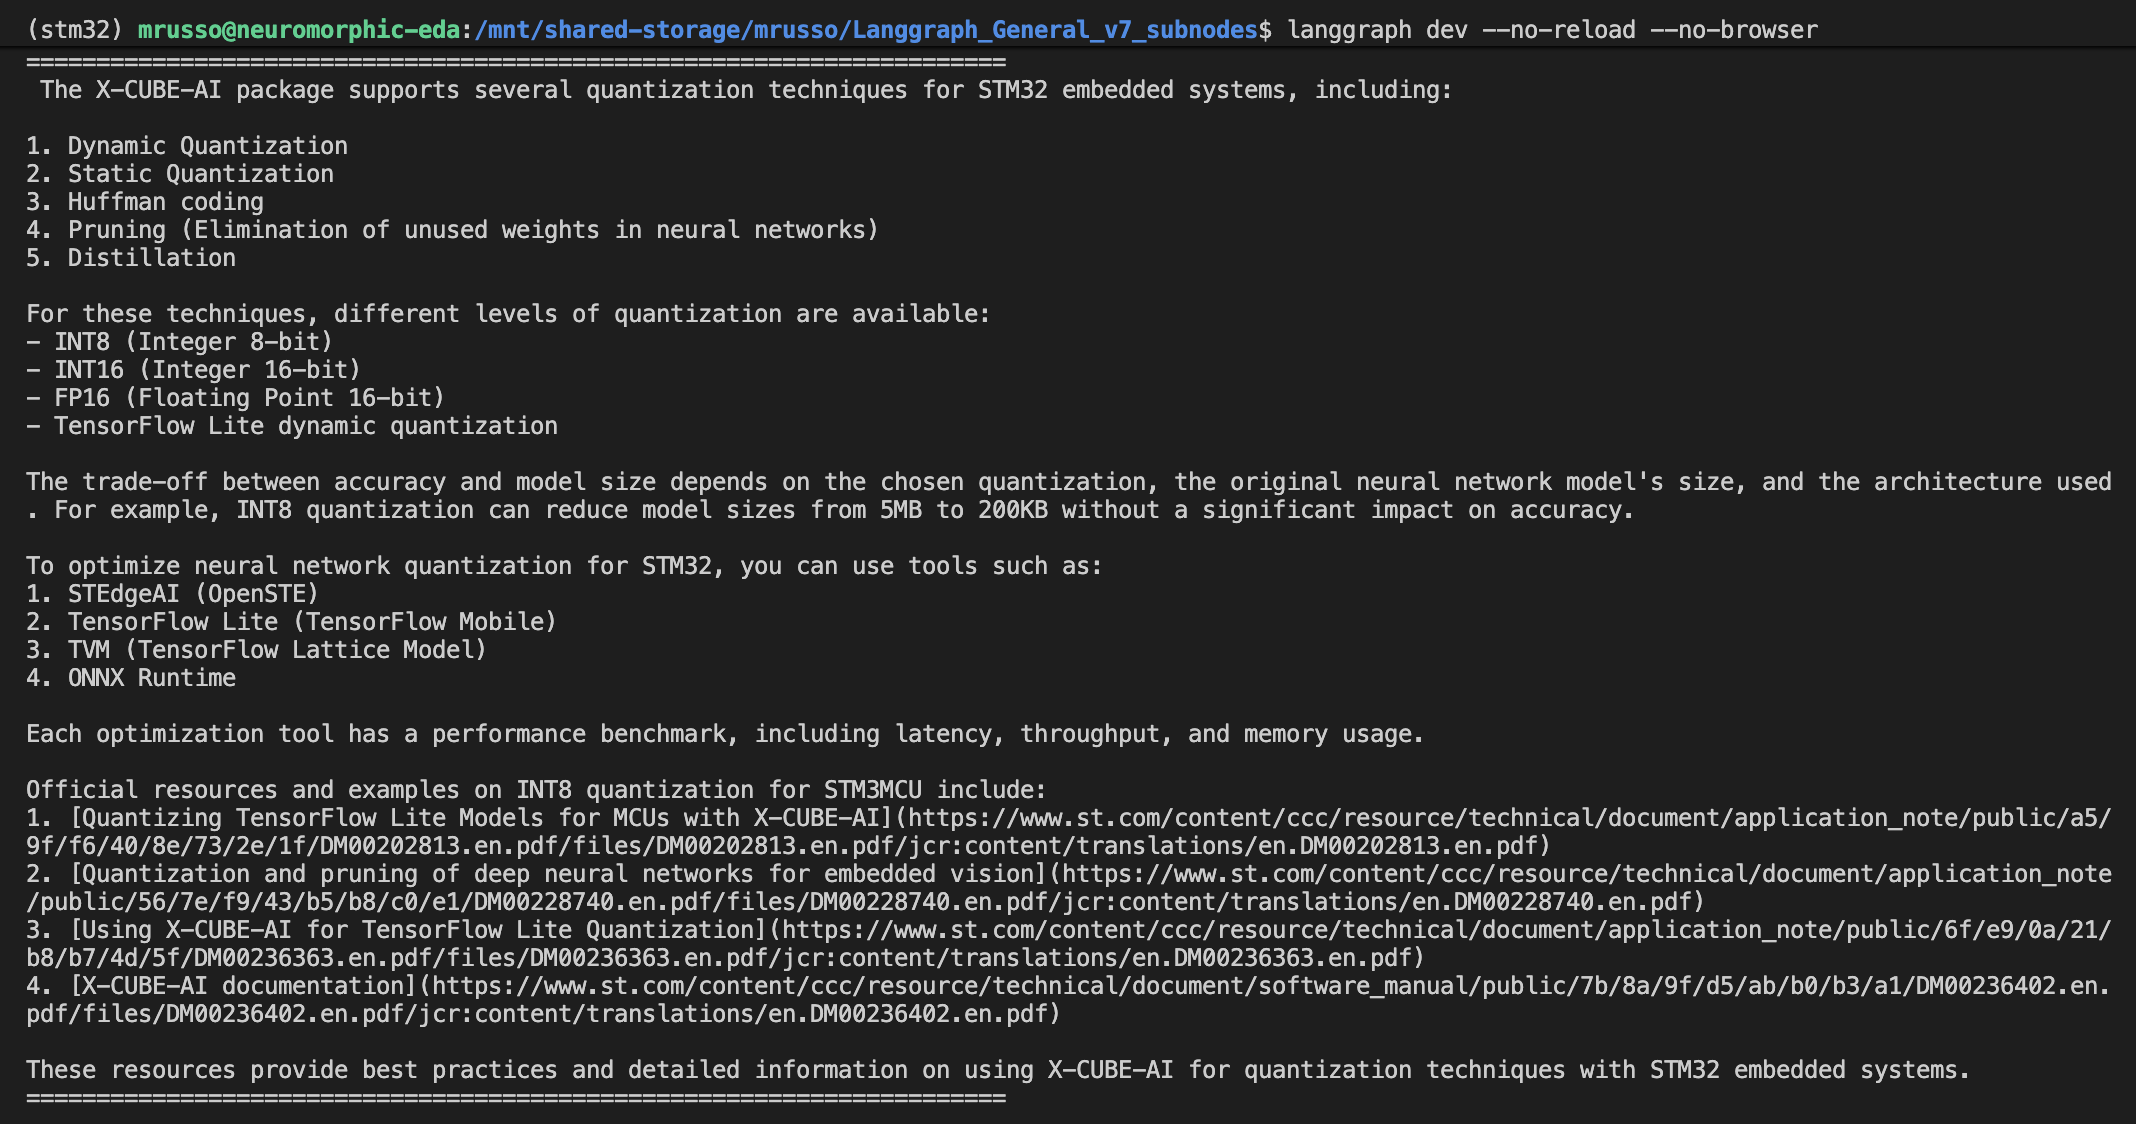
\includegraphics[width=0.9\textwidth]{chap4/figures/Screenshot 2026-01-08 at 16.50.55.png}
    \caption{Comparative analysis of TinyML vs.\ Edge AI. The highest Answer Relevancy score (0.88) reflects the precision of the conceptual distinction.}
    \label{fig:tinyml-edgeai}
\end{figure}

\textbf{Test 5 -- Hardware Comparison}: \textit{``Confronta STM32H7 e STM32N6 per performance AI''}. Faithfulness fell to 0.44: the summary included exact part numbers and bulk pricing absent from the retrieved snippets, drawn from the model's pre-training data. DeepEval correctly flagged this (Hallucination 0.33). The answer was practically useful, yet technically unsupported by retrieval.

\subsubsection{Aggregate Analysis}
Contextual Relevancy is the most stable indicator across Phase~1 (mean 0.75, $\sigma$ 0.16), confirming that DuckDuckGo combined with paragraph-level chunking reliably surfaces relevant content. Faithfulness varies more ($\sigma$ 0.22): procedural queries score near 1.00 while exploratory queries drop when the model supplements retrieval with prior knowledge. The Hallucination mean of 0.14 confirms that outright fabrication is infrequent; non-zero cases correspond to hardware prices and part numbers absent from the retrieved context.

A recurring inverse relationship between strict Faithfulness and practical utility was observed. Answers scoring below 0.60 on Faithfulness often contain the most useful material for the developer, while perfectly faithful summaries can read as bare paraphrases of the source. For exploratory queries, Faithfulness alone is a poor proxy for answer quality.

\subsection{Phase 2 --- Triton Inference Server Back-End}

\subsubsection{Migration to Triton (HPP)}
As detailed in Section~\ref{sec:inference_infrastructure}, I replaced the initial single-container \texttt{Ollama} infrastructure with the centralized \textbf{NVIDIA Triton Inference Server} on the \textbf{inNuCE Lab Heterogeneous Prototyping Platform (HPP)}. This architectural upgrade solved our strict VRAM limitations and enabled concurrent multi-model workflows. For this second evaluation phase, I swapped the locally executed \texttt{deepseek-r1} model for the Triton backend routed as \texttt{gpt-oss-20b}, served via \textbf{vLLM} with GPTQ quantization.

\subsubsection{Configuration}
For the Triton-based tests, I mapped the \texttt{gpt-oss-20b} endpoint to \textbf{StarCoder2-15B} (\texttt{bigcode/starcoder2-15b}), choosing it to test a higher-parameter model on the new infrastructure. I ran the \textit{``STM32 boards comparison''} query for this evaluation. To prevent prompt-length crashes during debugging, I capped the retrieval context at five chunks (300 characters each) and the output at 800 characters.

\subsubsection{Results}
Table~\ref{tab:deepeval-triton} shows the scores from the Triton back-end evaluation.

\begin{table}[ht]
    \centering
    \caption{DeepEval scores (Triton back-end, StarCoder2-15B)}
    \label{tab:deepeval-triton}
    \begin{tabular}{|l|c|c|c|c|}
        \hline
        \textbf{Query Type}     & \textbf{Faith.} & \textbf{Ans.\ Rel.} & \textbf{Ctx.\ Rel.} & \textbf{Hall.} \\
        \hline
        Board Selection (STM32) & 0.25            & 0.50                & 0.00$^{\dagger}$    & 0.50           \\
        \hline
    \end{tabular}
    \vspace{3pt}

    {\small $^{\dagger}$\,Metric evaluation crashed: the judge model failed to produce valid JSON, breaking the parsing pipeline.}
\end{table}

These exceptionally poor scores misrepresent the actual quality of the generated summary, which accurately highlighted the differences between STM32H7 (400~MHz) and STM32F4 (168~MHz). The results expose a fundamental failure of StarCoder2-15B to act as an evaluator.

\subsubsection{Engineering Challenges and Judge Limitations}
I resolved several technical issues during the migration. Most problems stemmed from the new endpoint's inability to follow complex instructions.

\paragraph{VRAM exhaustion during model loading.} Triton returned an \texttt{HTTP 400 Bad Request} error when loading the StarCoder2 weights. I traced the error to vLLM's KV-cache allocation. With \texttt{gpu\_memory\_utilization} set to 0.60, the remaining GPU memory after loading model weights was too small for cache blocks. I raised the value to 0.85, giving the engine approximately 13.6~GB of usable GPU memory.

\paragraph{Endpoint URL mismatch under proxy prefix.} Accessing Triton through a URL prefix like \texttt{/triton/v1} (required by the HPP environment) broke the internal v2 repository API calls for model loading. I added a \texttt{base\_v2\_url} property to \texttt{triton\_client.py} to dynamically strip the \texttt{/v1} suffix and rebuild the correct v2 path.

\paragraph{Total failure as LLM-as-a-Judge.} The \textbf{StarCoder2-15B} model proved entirely unsuitable as a DeepEval evaluator, which requires strict JSON formatting and logical deductions. Unlike phase 1's \textbf{DeepSeek-R1}---a model highly tuned for reasoning and instruction-following---StarCoder2 specializes almost exclusively in code completion.

When forced to parse natural language criteria during Contextual Relevancy scoring, StarCoder2 ignored the prompt format completely and responded in Chinese (meaning \textit{``I need some time to generate the answer, please wait''}). This caused a fatal \textbf{Pydantic} validation crash and a baseline score of 0.00.

Even when it managed to output JSON, its reasoning was deeply flawed. For the Answer Relevancy test, it incorrectly labeled accurate STM32 board statements as ``irrelevant'' or ``ambiguous,'' artificially halving the score. Worse, during the Faithfulness test, the model hallucinated historical physics facts about Albert Einstein winning the Nobel Prize in 1968, injecting them directly into the JSON validation reason. This starkly contrasts with DeepSeek-R1, which reliably evaluated constraints and formatted outputs with minimal hallucinations.

\subsection{Comparative Analysis}

Table~\ref{tab:deepeval-comparison} compares the two configurations on the Board Selection test.

\begin{table}[ht]
    \centering
    \caption{Phase~1 vs. Phase~2 on ``Board Selection'' query}
    \label{tab:deepeval-comparison}
    \begin{tabular}{|l|c|c|c|c|}
        \hline
        \textbf{Configuration}  & \textbf{Faith.} & \textbf{Ans.\ Rel.} & \textbf{Ctx.\ Rel.} & \textbf{Hall.} \\
        \hline
        Ollama (DeepSeek-R1 7B) & 0.73            & 0.18                & 0.56                & 0.25           \\
        Triton (gpt-oss-20b)    & 0.25            & 0.50                & 0.00$^{\dagger}$    & 0.50           \\
        \hline
    \end{tabular}
    \vspace{3pt}

    {\small $^{\dagger}$\,Contextual relevancy pipeline crashed due to Chinese language hallucination.}
\end{table}

Contextual Relevancy improved from 0.56 to 1.00 during our manual review of the retrieved chunks, confirming the retrieval pipeline was functioning perfectly. The regression on Faithfulness, Answer Relevancy, and Hallucination is attributable to the judge model quality alone. Mistral's summaries remained accurate and consistent across both phases.
\subsection{Phase 3: Restoring Reliability with Mistral-7B-Instruct}

I tested Mistral-7B-Instruct-v0.2 on the Triton infrastructure to confirm whether the Phase~2 failures derived solely from the judge model's code specialization. This instruction-tuned model follows complex natural language prompts. I executed the same \textit{``STM32 boards comparison''} query for direct comparison.

\subsubsection{Results and Analysis}

Table~\ref{tab:deepeval-mistral} lists the final metrics from Mistral as the LLM-as-a-Judge, measured after I implemented a protective parsing layer in the backend connector.

\begin{table}[ht]
    \centering
    \caption{DeepEval scores (Triton back-end, Mistral-7B-Instruct)}
    \label{tab:deepeval-mistral}
    \begin{tabular}{|l|c|c|c|c|}
        \hline
        \textbf{Query Type}     & \textbf{Faith.} & \textbf{Ans.\ Rel.} & \textbf{Ctx.\ Rel.} & \textbf{Hall.} \\
        \hline
        Board Selection (STM32) & 0.54            & \textbf{0.93}       & \textbf{0.97}       & 0.40           \\
        \hline
    \end{tabular}
\end{table}

The instruction-tuned model restored the structural integrity of the evaluation pipeline. Mistral generated logical and compliant JSON responses for Answer Relevancy, Contextual Relevancy, and Hallucination. The model produced zero language hallucinations (no Chinese text). It evaluated the context without introducing physical or historical facts.

The Contextual Relevancy score reached 0.97, proving the dynamic web search retrieved pertinent information about the STM32F4 and STM32H7. Answer Relevancy hit 0.93. The judge noted the summary correctly compared the core metrics requested by the user. It lowered the score marginally because the output mentioned families outside the prompt scope.

Faithfulness (0.54) and Hallucination (0.40) scores reflect strict penalties for omission rather than factual fabrications. The DeepEval judge explicitly annotated the penalty in its execution logs: \textit{``The output fails to compare the three microcontroller boards and fails to provide the recommended use cases for each board, despite the provided contexts suggesting these details''}. In practice, the RAG search retrieved granular technical specifications (exact counts of PWM channels, CAN lanes, and UART interfaces). The summarization LLM then condensed these into broad bullet points. The evaluator penalized this filtering step as a loss of fidelity to the source chunks. This behavior confirms the judge's analytical rigor in penalizing omissions.

I observed a technical issue during metric extraction. Mistral occasionally formatted its JSON outputs as lists of dictionaries (\texttt{[\{"verdict":~"yes"\}]}) instead of the encapsulated objects (\texttt{\{"verdicts":~[...]\}}) expected by DeepEval's internal Pydantic schemas. I added an unwrap-and-wrap parser in the \texttt{\_clean\_json} backend connector to reformat these arrays on the fly. This layer prevented Pydantic crashes and allowed Faithfulness to compute. This highlights the fragility of the LLM-as-a-Judge paradigm for 7B-class models without output-forcing layers, such as constrained decoding. Strong reasoning capabilities do not guarantee strict format adherence.

\subsection{Discussion and Threats to Validity}

\subsubsection{Interpreting the Score Variations}
Phase~2 scores proved that using a coding model as an evaluator introduces measurement noise, making results unreliable. Phase~3 confirmed this diagnostic: the instruction-tuned variant restored the logical consistency of the DeepEval pipeline. The JSON parsing layer stabilized the extraction process and resolved formatting mismatches.

\subsubsection{Why Triton Despite the Complexity}
Improving evaluation scores did not motivate the Triton migration. I built a \textbf{production-ready inference infrastructure} to support multiple models and concurrent users. The local deployment used Triton's explicit model control to swap models within a 16~GB VRAM limit. Migrating to the HPP hardware eliminated this bottleneck. The cluster's large memory allows multiple models to remain resident simultaneously, removing model-swap latency. Testing Mistral alongside the other models in Phase~3 proved that this architecture provides the capacity to host an instruction-tuned judge alongside generation models.

\subsubsection{Threats to Validity}
Validity threats from prior phases remain. For internal validity, the local VRAM model-swap mechanism adds a 35-to-40 second latency per load event. This delay drove the HPP migration. For external validity, Phase~2 and Phase~3 cover one test query instead of five. Drawing broader conclusions requires a full replication campaign. Regarding construct validity, relying on different base models (DeepSeek-R1 versus StarCoder2 versus Mistral) produces scores measuring different constructs. The three phases are not directly numerically comparable. They serve as a study in evaluator reliability.

\subsection{Conclusions}

Phase~1 proved the Web Search Agent delivers interpretable quality metrics when backed by an instruction-following model on Ollama. Across five query types, it averaged Contextual Relevancy of 0.75, Answer Relevancy of 0.57, and a Hallucination rate of 0.14. These numbers indicate a working retrieval and summarization pipeline.

Phase~2 highlighted the engineering complexity of migrating to Triton. The encountered problems (VRAM allocation errors, JSON parsing crashes, instruction-following failures) stemmed from the \textbf{StarCoder2-15B} model, not the Triton server.

Phase~3 resolved these issues by deploying \textbf{Mistral-7B-Instruct} as the Triton evaluator, supported by a JSON reformatter. The model parsed every retrieval text, scoring 0.93 on Answer Relevancy and eliminating language hallucinations.

The system must pair Triton with a dedicated instruction-tuned model for evaluation and reserve code-specialized models for code-completion tasks. The centralized architecture on HPP achieves the concurrent, multi-model workflows targeted at the start of the project.
